\subsection{20 августа. пер. Уллукёль Восточный (1А*)}
\textit{Метеоусловия: утром, днём ясно, вечером~--- переменная облачность, тепло.}

\begin{figure}[h!]
	\centering
	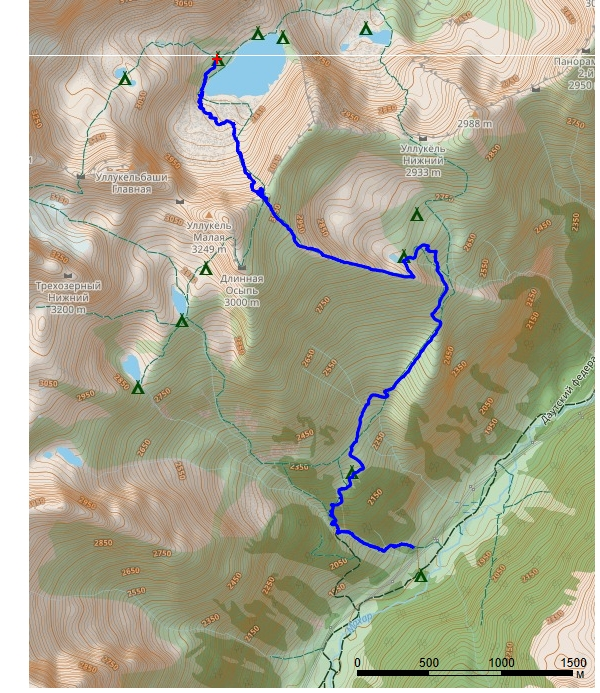
\includegraphics[angle=0, width=0.7\linewidth]{../pics/mini_maps/20}
	\label{fig:mini_20}
\end{figure}

Подъём дежурных в 04:30, общий подъём в 05:00. Выход группы в 07:30. Движемся по разведанному вчера маршруту по крупной осыпи в обход южной оконечности озера. На одном из привалов участнице (Наташе Мироновой) становится нехорошо, и часть пути (ок. 15 мин. ЧХВ) она проходит без рюкзака. Пока доносим рюкзак, группа фотографируется на фоне озера (рис.~\ref{fig:DSC_0907}).

Далее движемся по моренному гребешку и выходим на среднюю осыпь перевального взлёта, прижимаясь к правому пхд борту кулуара..

\begin{figure}[h!]
	\centering
	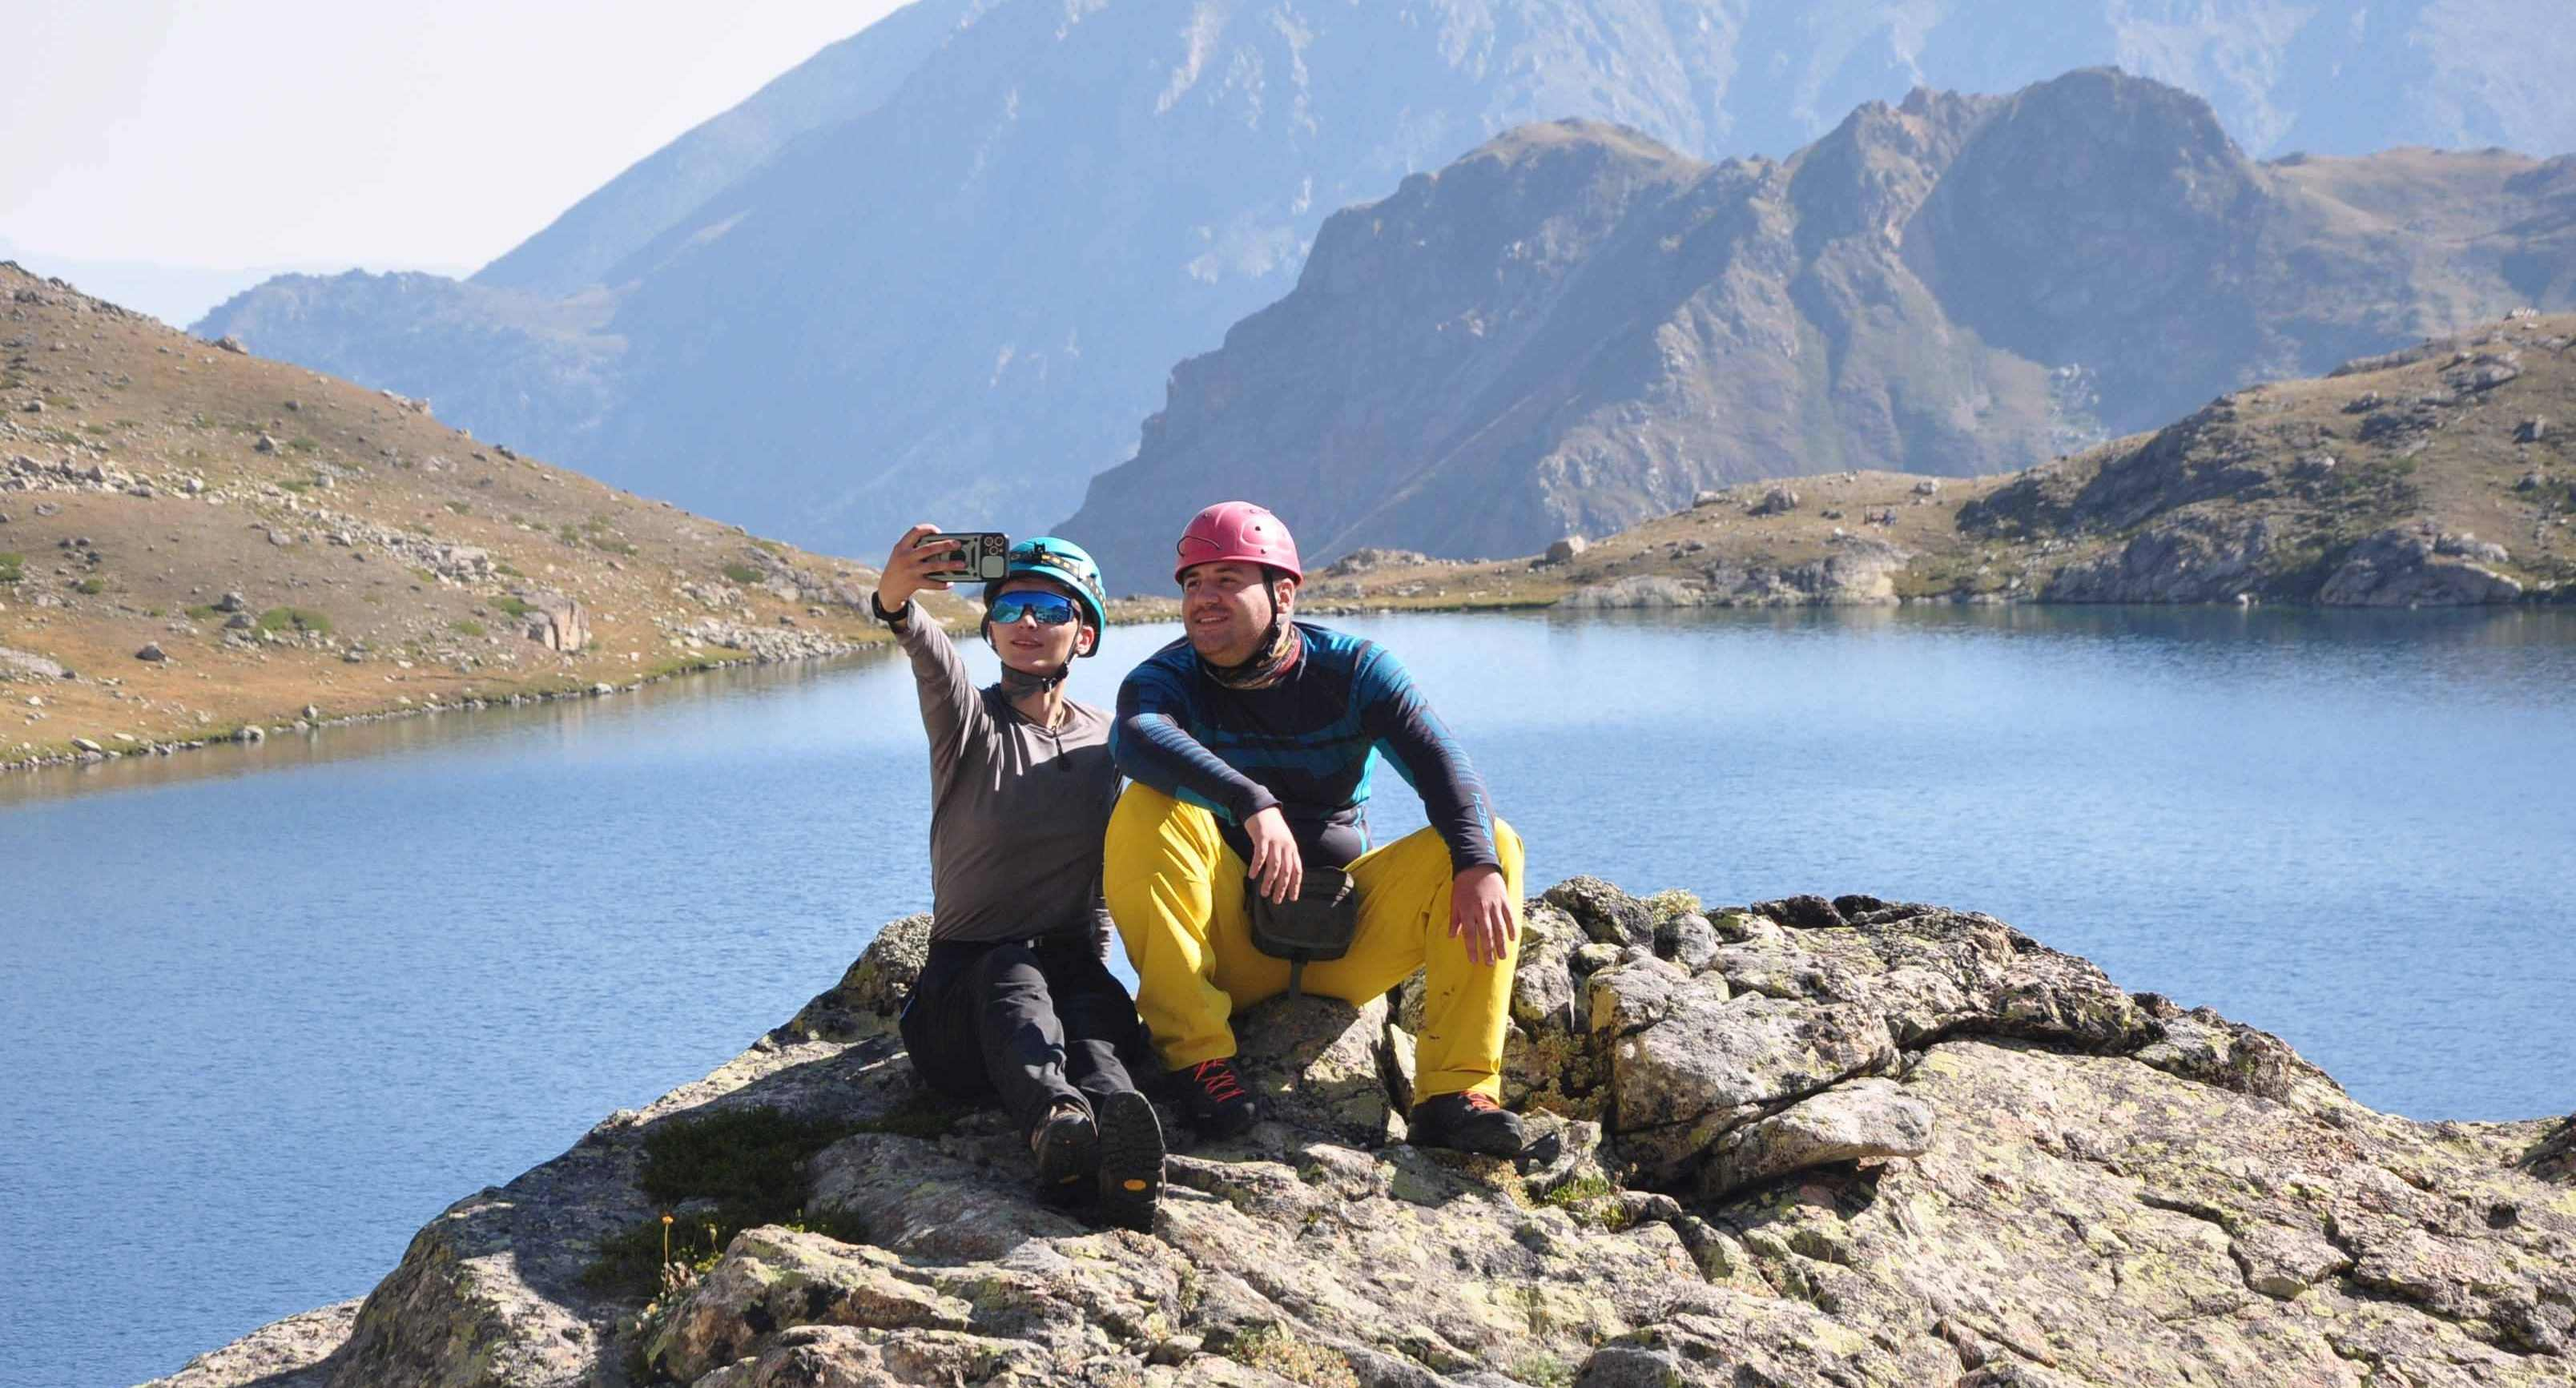
\includegraphics[width=0.7\linewidth]{../pics/DSC_0907}
	\caption{Фоткаемся на фоне озера}
	\label{fig:DSC_0907}
\end{figure}

\begin{figure}[h!]
	\centering
	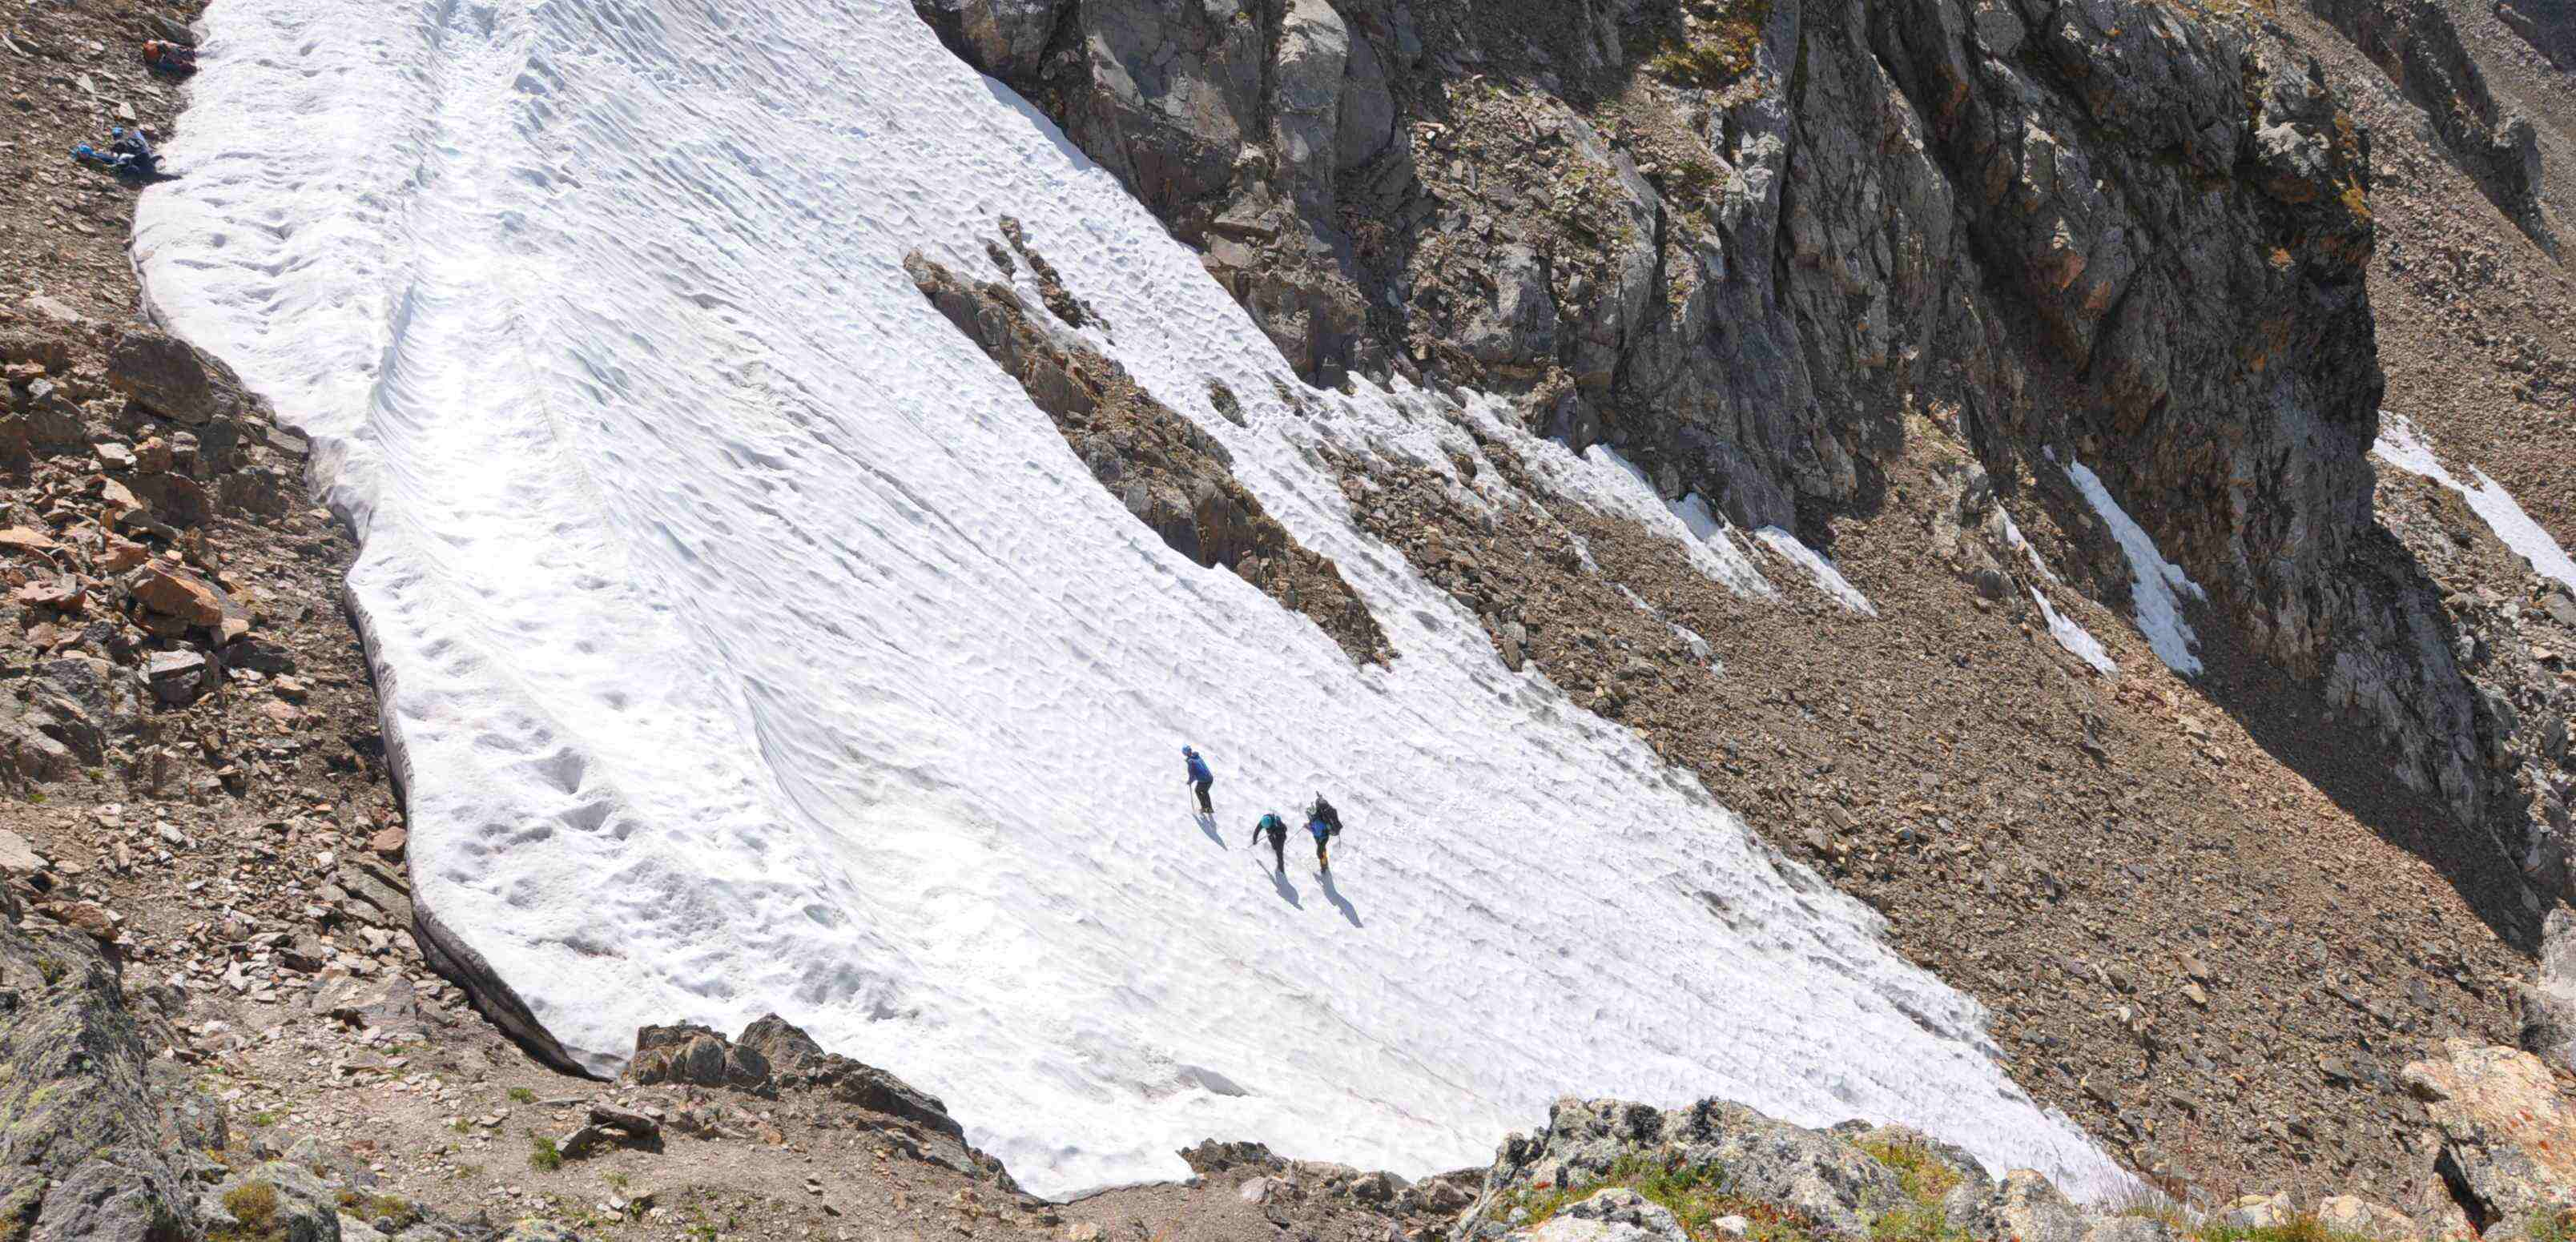
\includegraphics[width=0.7\linewidth]{../pics/DSC_0946.png}
	\caption{Маршрут движения группы по снежнику (красный), траектория срыва участника (синий), маршрут подъёма с сорвавшимся участником (чёрный)}
	\label{fig:DSC_0946}
\end{figure}


\begin{figure}[h!]
	\centering
	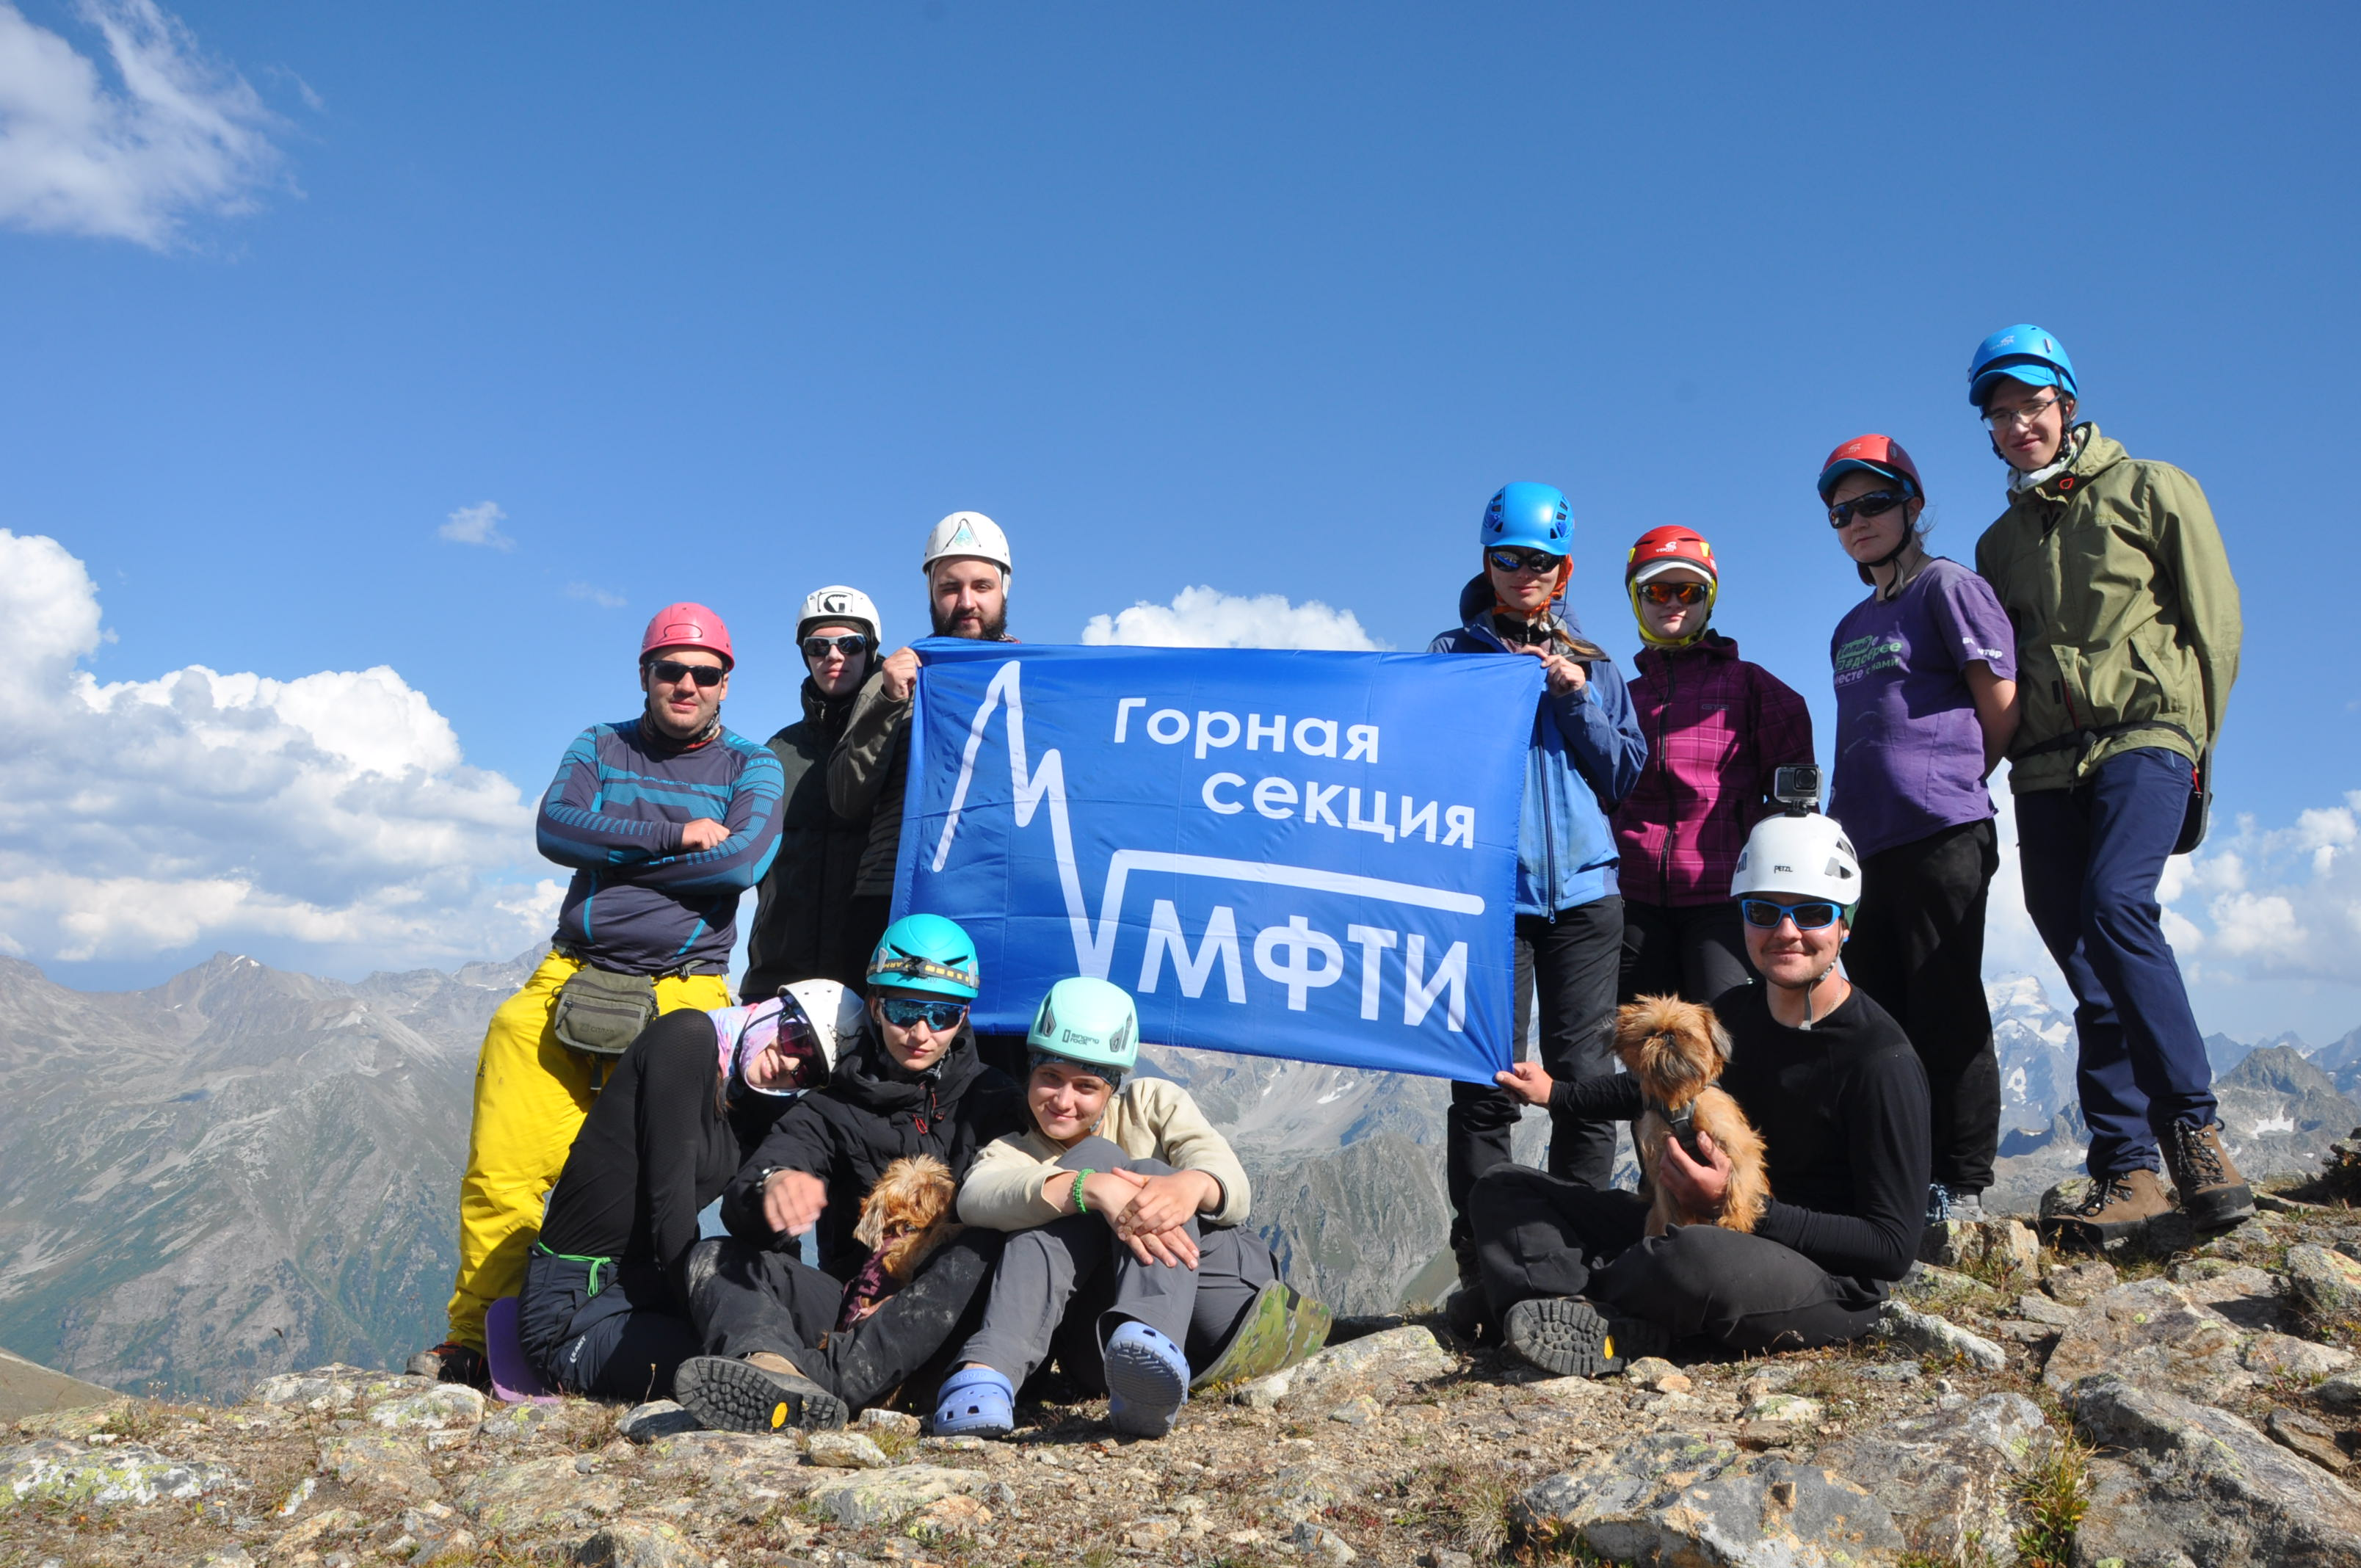
\includegraphics[width=0.7\linewidth]{../pics/DSC_0982}
	\caption{Группа на перевале, вид на д.р. Махар}
	\label{fig:DSC_0982}
\end{figure}

\begin{figure}[h!]
	\centering
	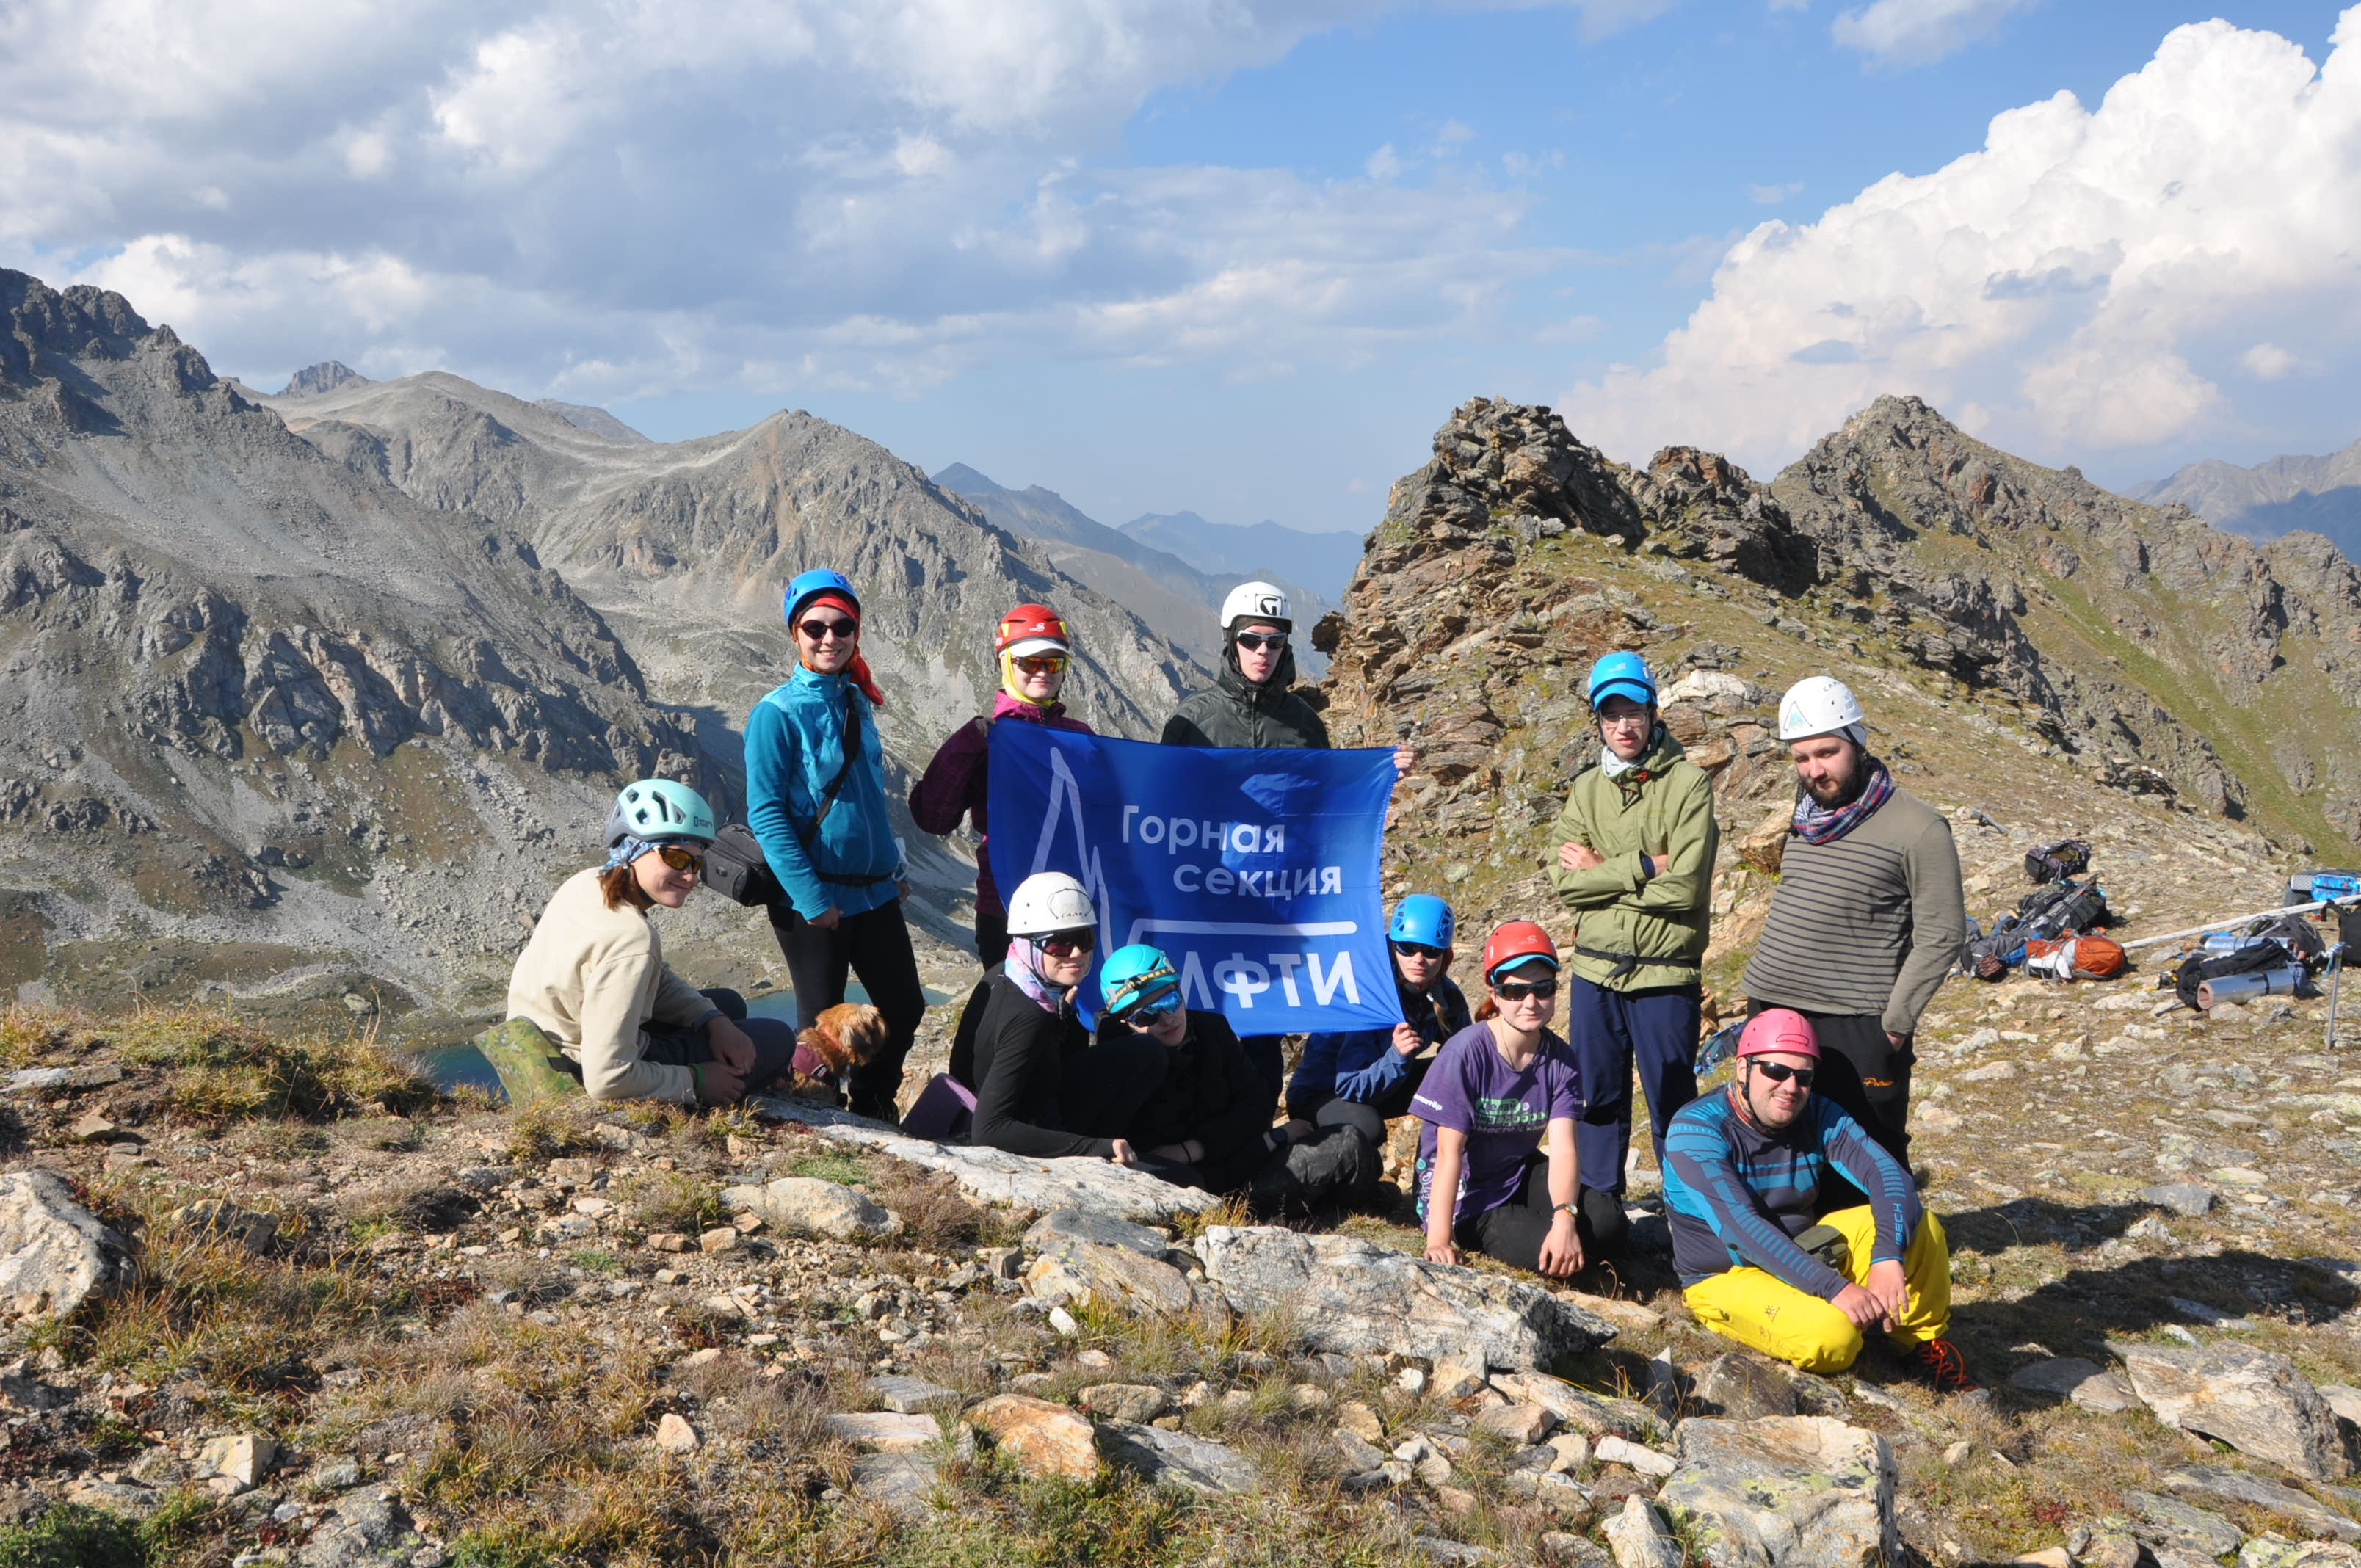
\includegraphics[width=0.7\linewidth]{../pics/DSC_0986}
	\caption{Группа на перевале, вид на оз. Уллу-Кёль}
	\label{fig:DSC_0986}
\end{figure}

\newpage